\section*{Corrections}

\textit{February 10, 2022} \\

Since publishing this report, the authors found two errors in the model inputs
that significantly change the results. First, Table \ref{tab:cost_table} reports
the correct technology fixed costs in millions of dollars per gigawatt-year.
However, the model requires fixed costs in millions of dollars per \textit{megawatt}-year.
Therefore, the fixed costs used in the original model were three orders of
magnitude too high. This gave the fixed costs an outsized influence on the model
and produced ``unphysical'' results for the objective function. Adjusting
the fixed costs affected both the objective function value and the model capacity
expansion. Figure \ref{fig:system_cost} shows the new levelized costs of
electricity for each scenario. Keeping Illinois' existing nuclear fleet open
through 2050 is the cheapest scenario in all cases. Figure \ref{fig:correct_capacity_2050}
shows the new capacity mix in Illinois in 2050.

\begin{figure}[H]
  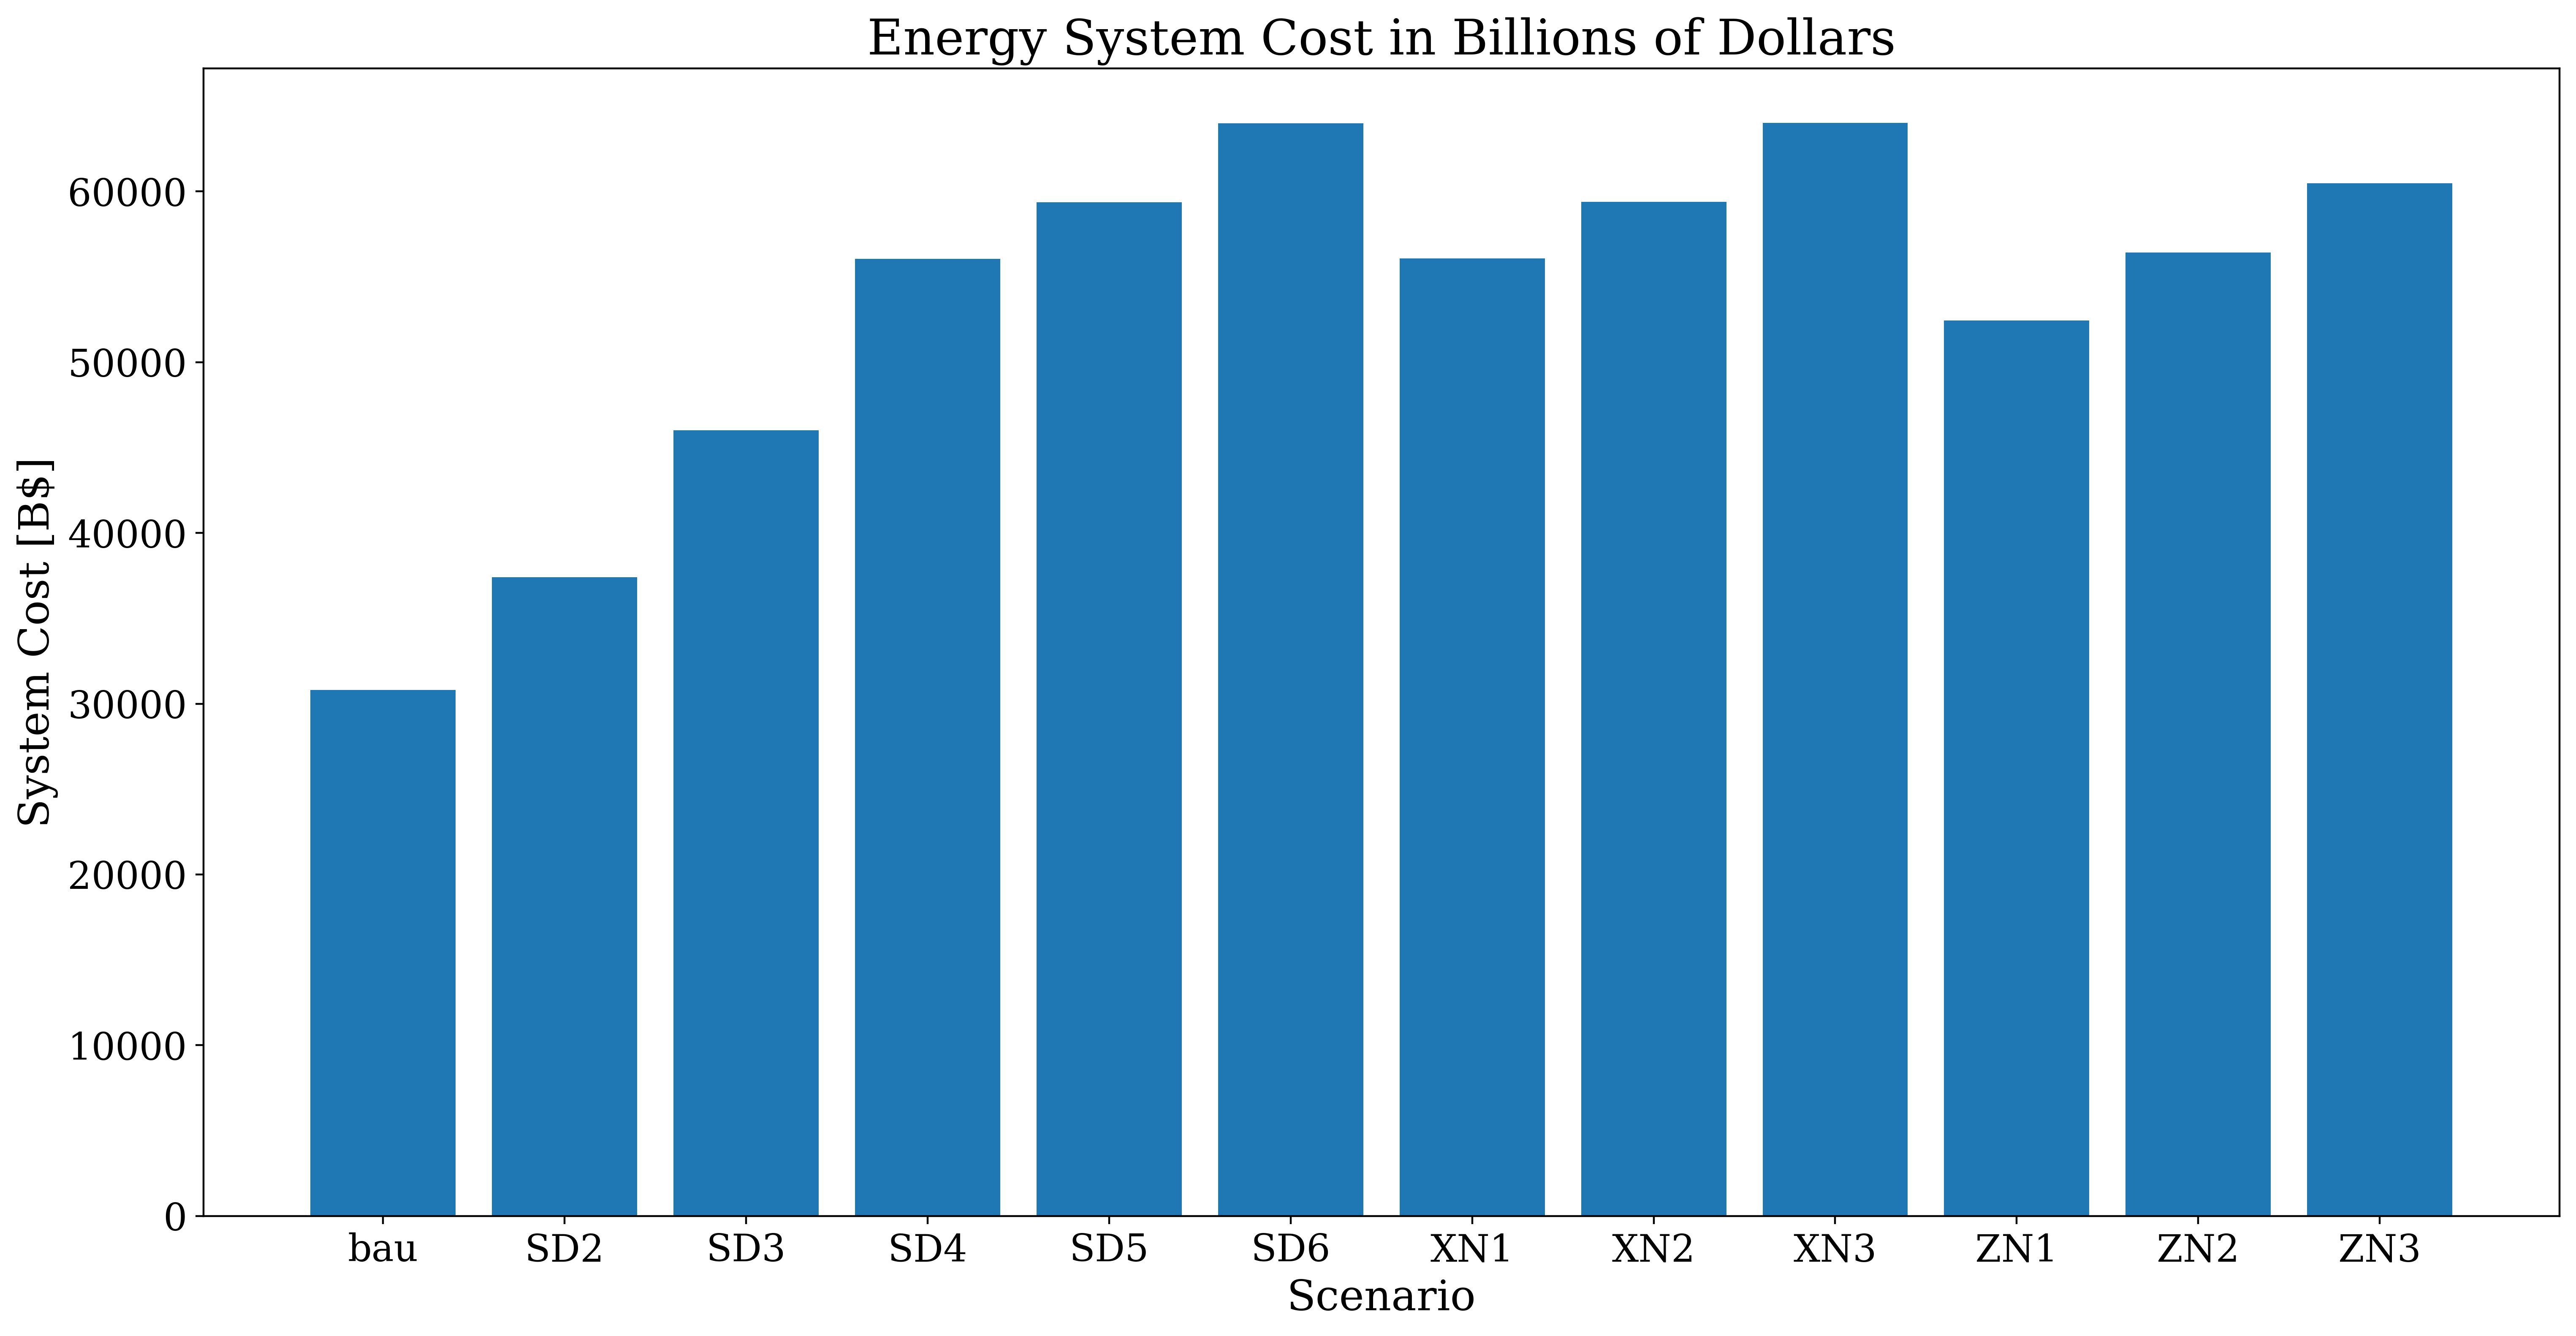
\includegraphics[width=\textwidth]{temoa_CORRECTED/total_system_cost}
  \caption{Compares the levelized cost of electricity for each scenario in this
  study.}
  \label{fig:system_cost}
\end{figure}

\begin{figure}[H]
  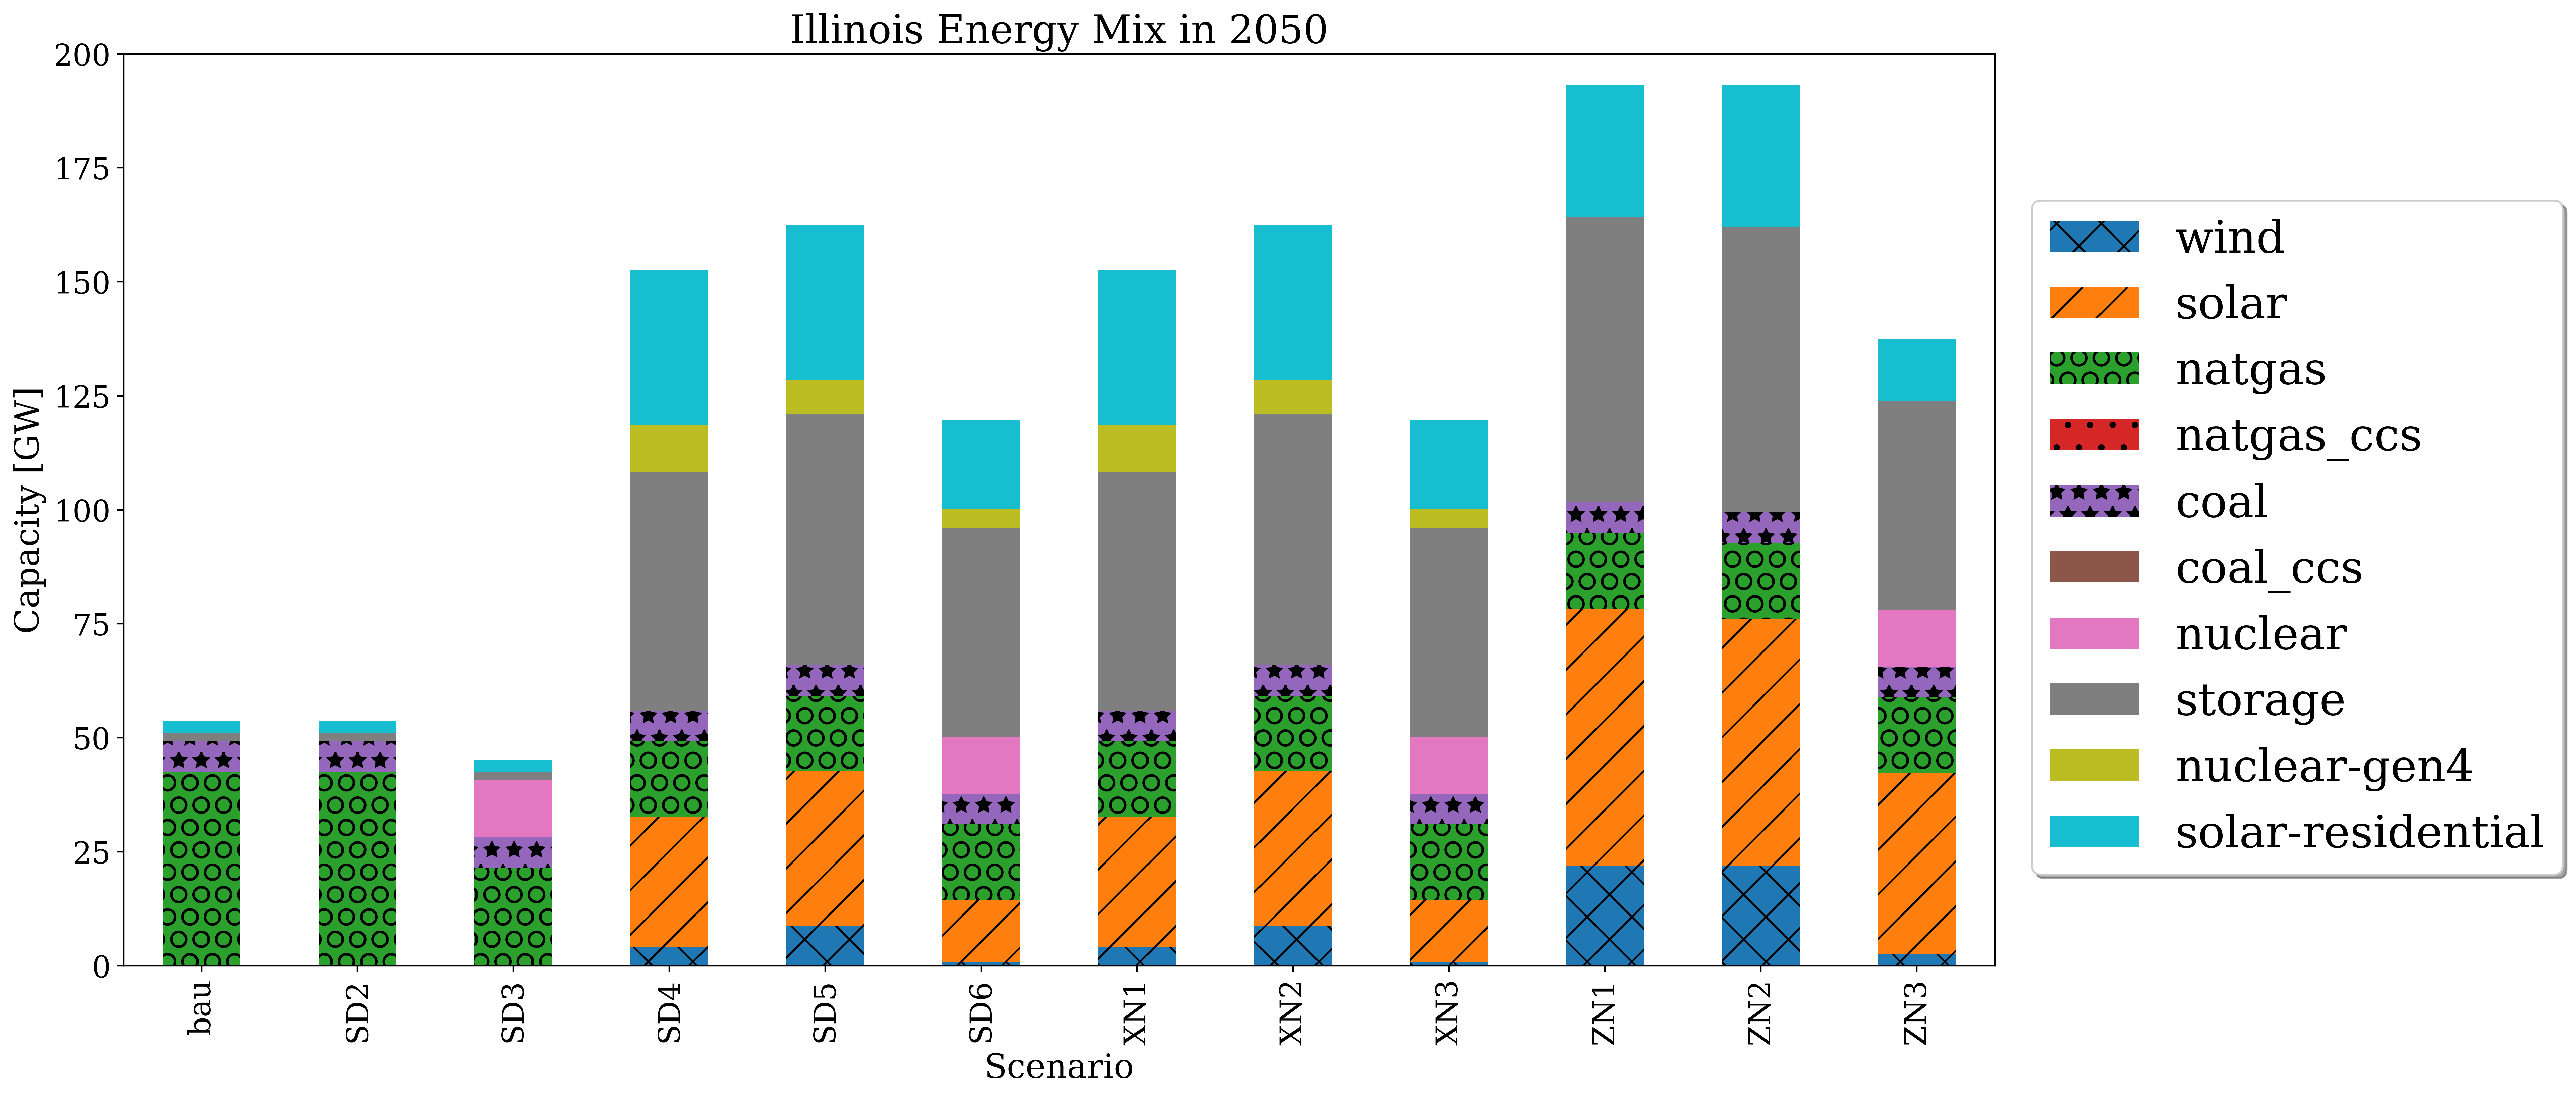
\includegraphics[width=\textwidth]{temoa_CORRECTED/final_capacity}
  \caption{Compares the final capacity mix for each scenario in this
  study by 2050.}
  \label{fig:correct_capacity_2050}
\end{figure}

Second, the power density values used to calculate land use change for each
scenario were originally taken from \cite{van_zalk_spatial_2018}, which reports
\textit{the area required to produce 1 MW equivalent.} Thus, those values
already incorporated capacity factor for each technology and the original
results in this report double-counted the capacity factor for solar and wind
generators. Figure \ref{fig:landuse_correct} shows the corrected land use change.
Due to changes in capacity mix, more land is devoted to wind power in the nuclear-constrained
scenarios.

\begin{figure}[H]
  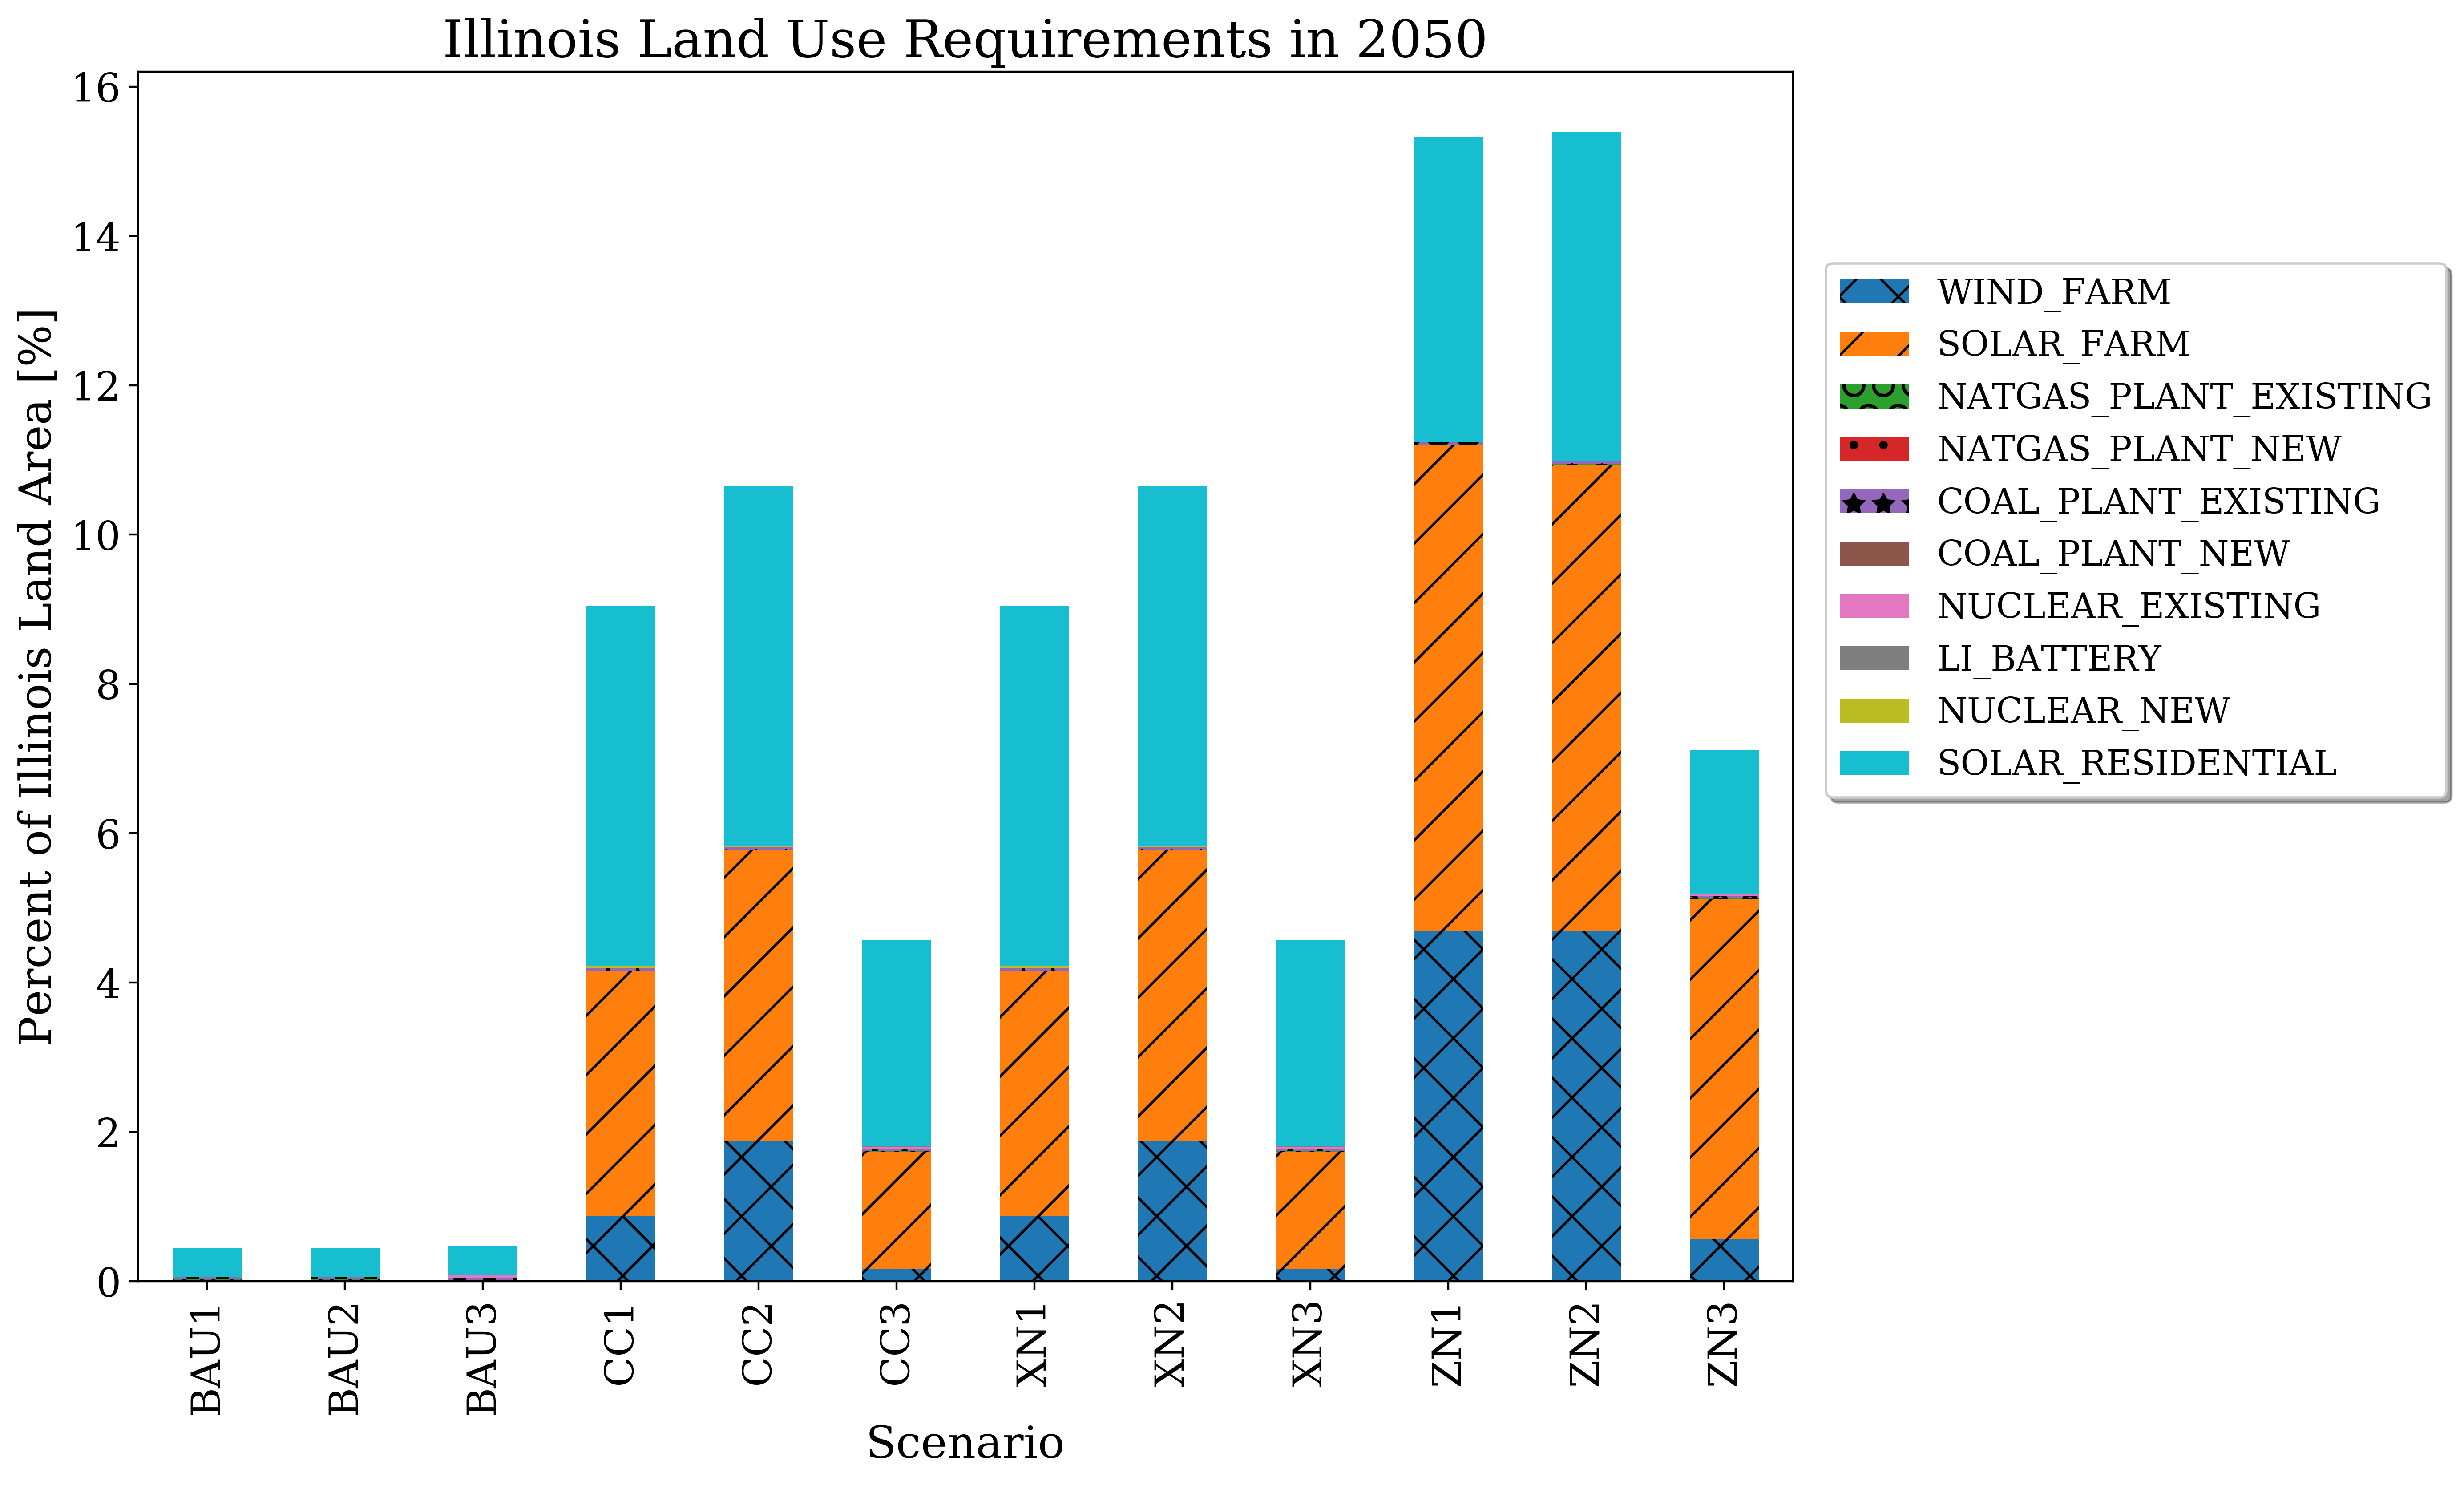
\includegraphics[width=\textwidth]{temoa_CORRECTED/total_landuse_percentage}
  \caption{Compares the land use change for each scenario in this
  study by 2050.}
  \label{fig:landuse_correct}
\end{figure}

These changes also influence the study takeaways. The study now demonstrates:
\begin{itemize}
  \item nuclear energy is necessary to reach Illinois' carbon reduction goals;
  \item without existing nuclear power, reaching zero carbon would require
  \textit{wind} deployments to displace \textit{12,500 km$^2$} of critical Illinois
  farmland;
  \item deploying new advanced nuclear generation is the least expensive way to allow
  Illinois farmland to remain farmland \textit{and is the overall least expensive
  pathway to } reaching zero-carbon by 2030.
  \item Keeping Illinois' existing nuclear plants open through 2050 avoids
  \textit{nearly 5 million metric tons of life-cycle CO$_2$ per year} and
  \textit{150,000} metric tons of e-waste.
  \item Deploying advanced nuclear avoids approximately \textit{500,000} metric
  tons of e-waste.
  \item \textit{Without deploying advanced nuclear reactors, an extraordinary,
  possibly infeasible grid-scale battery storage capacity is required to meet
  any zero-carbon target.}
\end{itemize}
